\documentclass[onecolumn, letterpaper, ]{report}
\usepackage[utf8]{inputenc}
\usepackage{tabularx}
\usepackage{booktabs}
\usepackage[english]{babel}
\usepackage{graphicx}
\graphicspath{ {./images/} }
\usepackage{lipsum} 
\usepackage{tikz-uml}
\usepackage{dirtytalk}
\usepackage{geometry}
\usepackage{array}
\usepackage{rotating}
\usepackage{longtable}
\usepackage{pdflscape}

\usepackage{listings}
\usepackage{xcolor}

\definecolor{background}{HTML}{2E2E2E}
\definecolor{comment}{HTML}{3A9D23}
\definecolor{prompt}{HTML}{46AFC2}
\definecolor{output}{HTML}{D0D0D0}

\lstdefinestyle{custombash}{
    backgroundcolor=\color{background},
    basicstyle=\small\ttfamily\color{output},
    commentstyle=\color{comment},
    keywordstyle=\color{prompt},
    morekeywords={user@hostname:~\$},
    numbers=left,
    numberstyle=\tiny\color{output},
    showstringspaces=false,
    tabsize=4,
    lineskip=-1.5pt, % Add this line to adjust line spacing
}




%\usepackage{draftwatermark}
%\SetWatermarkLightness{ 0.9 }
%\SetWatermarkText{Jorge Alvarez}
%\SetWatermarkScale{ 5}


\usepackage{amsmath}
\usepackage{mathtools}


\begin{document}
 
  \title{University of Nevada, Las Vegas\\Lee Business School\\Department of Management, Entrepreneurship, and Technology\\ . \\MIS 768: Advanced Software Concepts\\ Project: Global Remittance System}
    \author{Philip Mensah & Jorge Alvarez &  &Han-fen Hu, Ph.D. \thanks{We give thanks to the Department of Management, Entrepreneurship,
and Technology of the Lee Business school for our education and support, as well as for making this project possible. We are grateful for Dr. Han-fen Hu, who is helping us along the way.} }
    \date{Spring 2024}

     \maketitle
    
        

   \tableofcontents
   



   
    \chapter{Project Proposal and Design.}

 


    \section{\colorbox{white!95!black}{Background}}
        In today's interconnected world, the movement of people across borders has become increasingly common. With this migration comes the need for individuals to send money back home to support their families and loved ones. Remittances, the transfer of money by foreign workers to their home countries, play a crucial role in the economic well-being of millions of families worldwide. However, the process of sending remittances can be complex, costly, and time-consuming, especially for those who are unfamiliar with banking systems or lack access to traditional financial services.

        Many individuals who rely on remittance payments may reside in remote areas or countries with limited banking infrastructure. Therefore, there is a need for a remittance system that is accessible to a wide range of users, regardless of their location or financial status. 
        
        Timeliness is crucial for remittance recipients who may rely on these funds for essential expenses such as healthcare, education, or daily living costs. A system that facilitates fast and efficient transfers will help ensure that recipients receive funds promptly.
        
        Remittance senders and recipients alike benefit from transparency regarding exchange rates, fees, and transaction status. Providing users with clear and comprehensive information about their transactions helps build trust and confidence in the system.
        
        The current landscape of remittance payments is marred by inefficiencies, high costs, and limited access, hindering the ability of individuals to send and receive money abroad effectively. Many people, particularly those in developing countries, face significant obstacles when trying to access formal financial services or transfer money across borders. Our goal is to develop a Java-based remittance app - RemitEase, to streamline the remittance process, reduce costs, improve accessibility, and enhance the overall user experience. This application will empower individuals to send and receive money securely and conveniently, thereby contributing to financial inclusion, poverty reduction, and economic development on a global scale.

        

    \section{\colorbox{white!95!black}{Function List:} } 
    Here is a closer look at the list of function we panned for our system. We explain its importance and how it contributes to the overall operation of the remittance system.

        \subsection{User Registration}
            New users can create an account that will link them personal information stored in the system. This account will have authentication requirements for access. To first create the account, they will provide essential personal information useful to the remittance process. This can be the name, email, phone number and address. We will implement an input validation system to ensure that the information provided is complete and error free. 
    
        \subsection{Update User} The user should be able to modify their personal information saved. This ensures that essential personal information is up-to-date. 

        \subsection{User Login} Access is granted according to the access level and user credential that are set up during the User registration process. This authentication check enhances security and user privacy by ensuring that access is granted only the account owner.

        \subsection{Transaction History} Allows the user to see a history of their transactions indexed by time. This allows options such as, repeat a transaction, view current status of a transaction.

        \subsection{Create Remittance} They can initiate a remittance payment to a recipient anywhere via our remittance network. User must input a recipient's name, address, and other contact information as well as the destination country. 

        \subsection{Calculate Fees} The fee is calculated based on the amount that is sent. 

        \subsection{Currency Converter} Uses logic and a market exchange rates to convert the remittance amount to the currency of the recipients' country. This will ensure a consistent and accurate conversion.

        \subsection{Process Remittance} Sends the remittance to appropriate partner in the remittance network. Sets the status to in progress.

        \subsection{Cancel Remittance} Allows the sender to cancel transactions that are in progress pending pickup. 

        \subsection{Receive Remittance} The partner institution disburses the remittance to the recipient. 

        \subsection{Add Partner} As our global reach grows new remittance partners can be added by system administrators.

        \subsection{Update Exchange Rates} Connects to an external API to obtain real time market foreign exchange rates. 

        \subsection{Partner Settlement} Calculate the amount owned to partners in the remittance network and settles these balances.

        \subsection{Send Notification} We can leverage Twillio SMS API to send transaction-related information to senders and recipients. We can notify them of confirmations of transfers and update their status when picked up.
    

    
    \begin{landscape}
        \section{\colorbox{white!95!black}{User Interface (UI) design:}}
    Provide a graphical representation of each function. The UI design should show a mock-up flow of using the system from start to finish.

    \subsection{Slpash Screen and Log-In}
        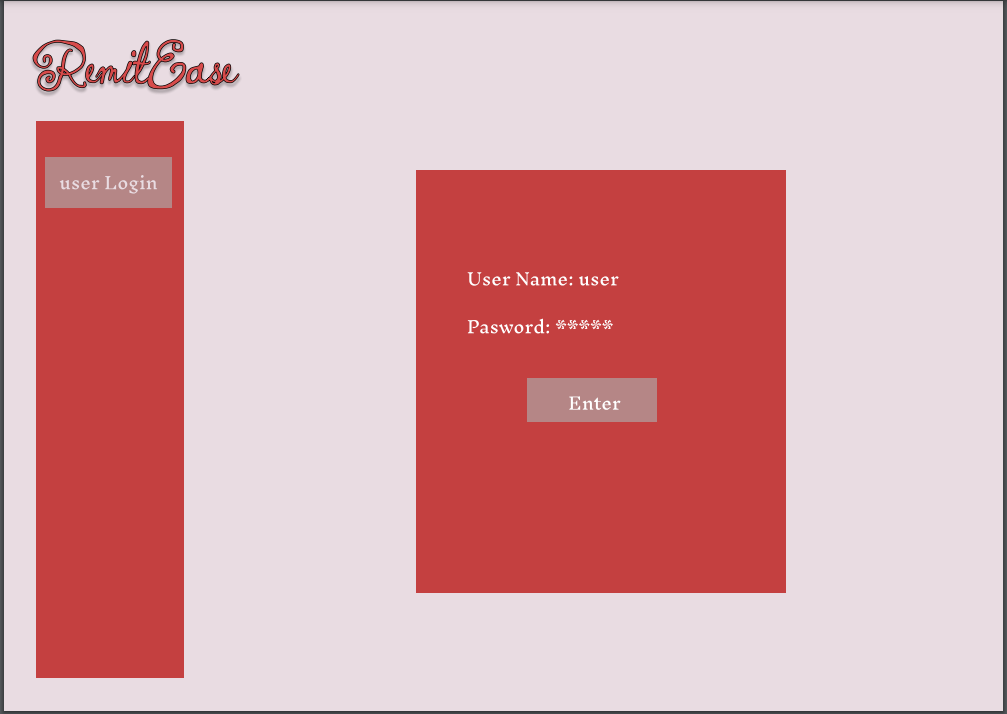
\includegraphics[width=.8\linewidth]{MockUps/login.PNG}
        
        A mockup of a login screen for an application named "RemitEase." The mockup presents a simple and user-friendly interface with the log in form.
    \end{landscape}

    \begin{landscape}
        \subsection{Welcome Screen- Main Menu}
        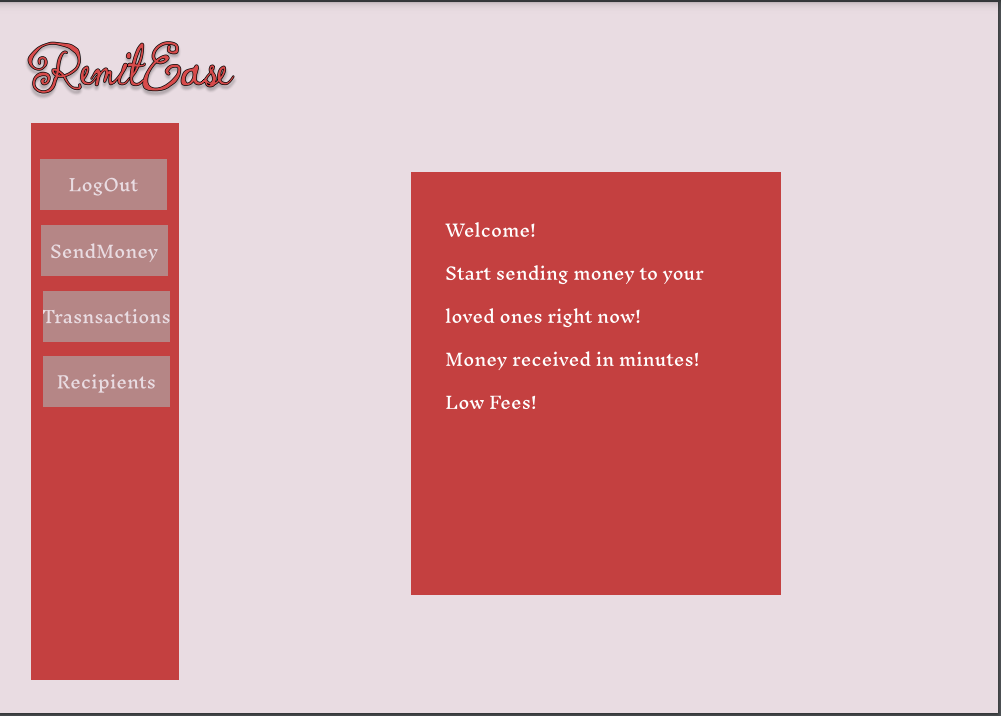
\includegraphics[width=1\linewidth]{MockUps/2welcome.PNG}

        Main screen with a navigation sidebar pointing to system functions.
    \end{landscape}

    \begin{landscape}
        \subsection{New Recipient Info form} 
        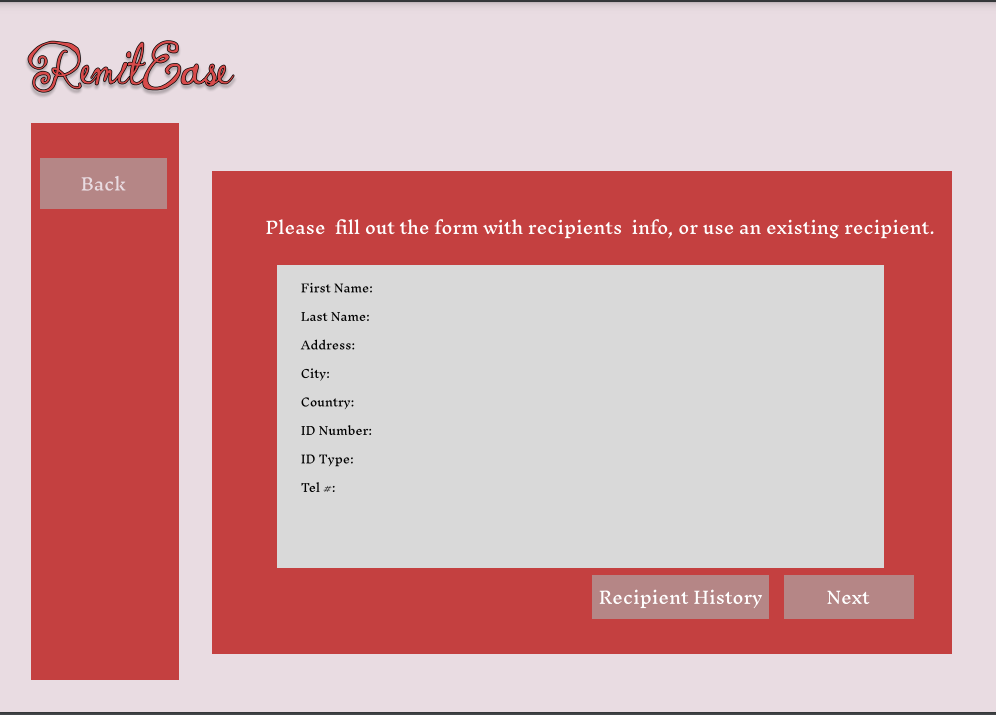
\includegraphics[width=.97\linewidth]{MockUps/3ReceipientsInfoForm.PNG} 

        Customer that initiates a new remittance has the function to add a new recipient.
    \end{landscape}
    
        
    \begin{landscape}
        \subsection{Amount input Screen}
        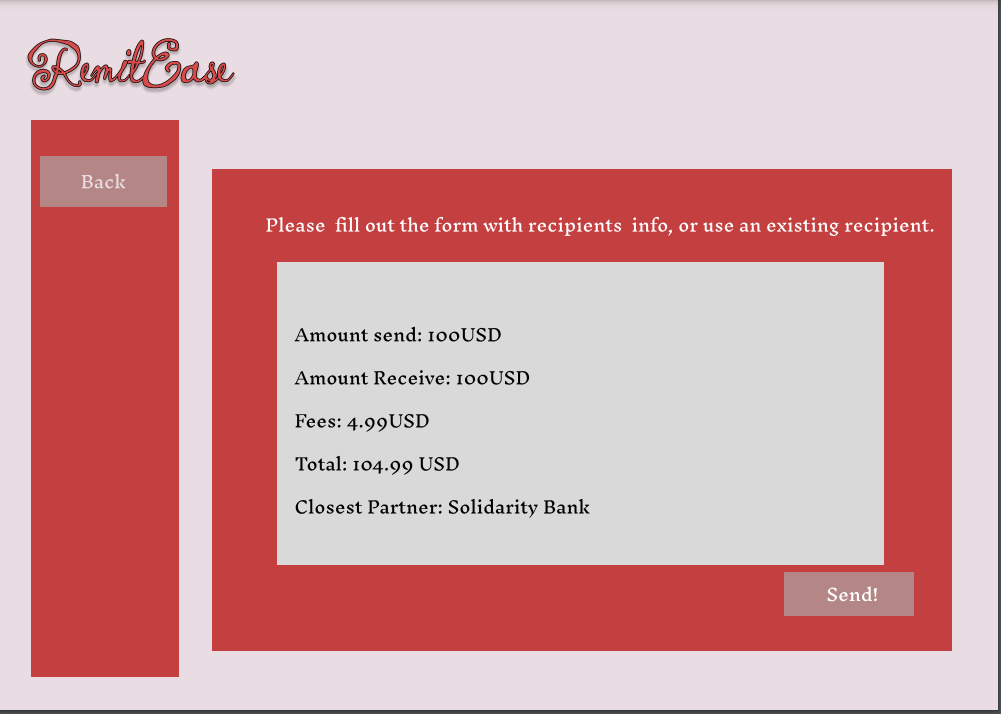
\includegraphics[width=.97\linewidth]{MockUps/AmountScreen.PNG}

        After recipient details are added, the program offers the function to input remittance amount. Then it shows receive amount in target currency and fees as a function of remittance amount.
    \end{landscape}

    \begin{landscape}
        \subsection{List of Saved Recipients}
        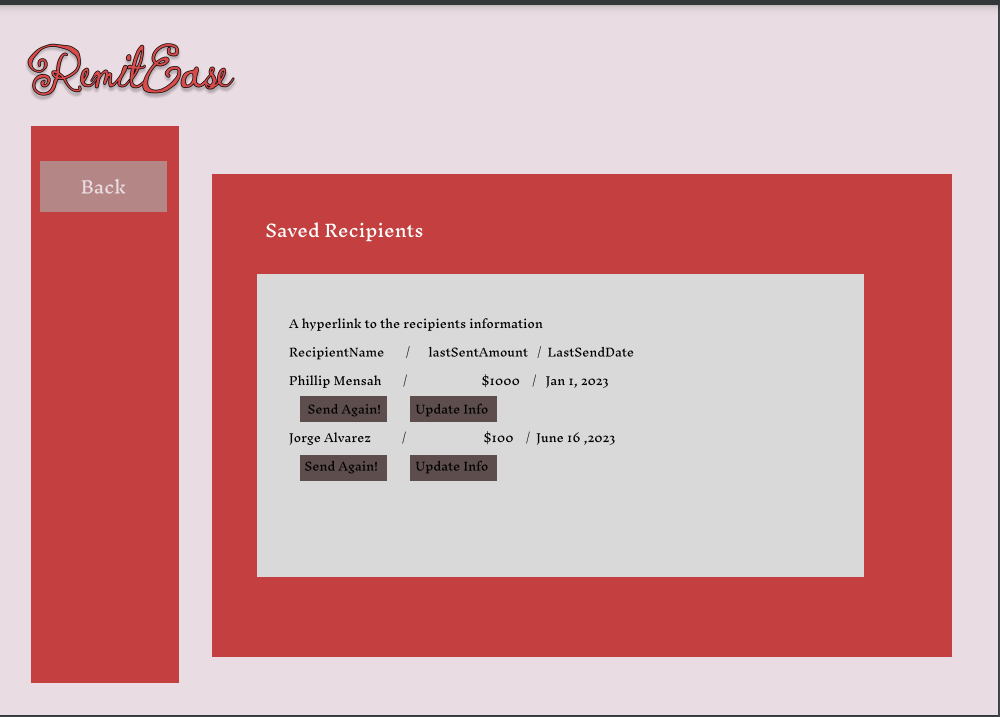
\includegraphics[width=.97\linewidth]{MockUps/Recipients.PNG}

        Function that shows the list of saved recipients and a function to send remittance or update/delete the saved recipient.
    \end{landscape}
    
    \begin{landscape}
        \subsection{Recipient Update Confirmation}
        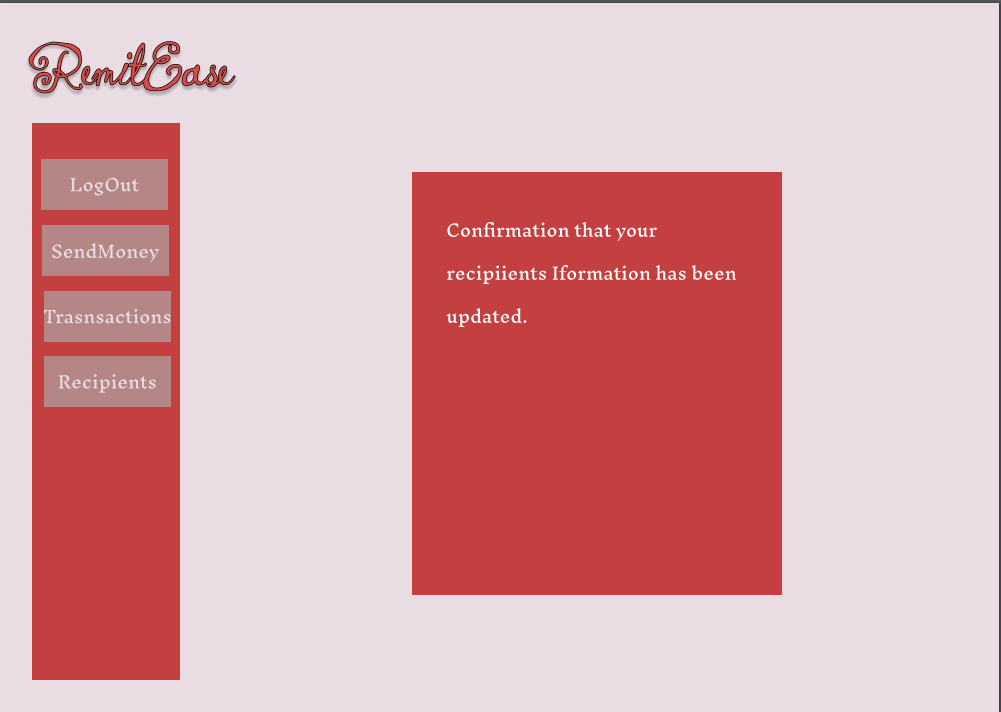
\includegraphics[width=.97\linewidth]{MockUps/RecipientUpdateConfirmation.PNG}
        
        Backend function has updated the recipient details. Front end shows confirmation.
    \end{landscape}

    \begin{landscape}
        \subsection{Send Confirmation}
        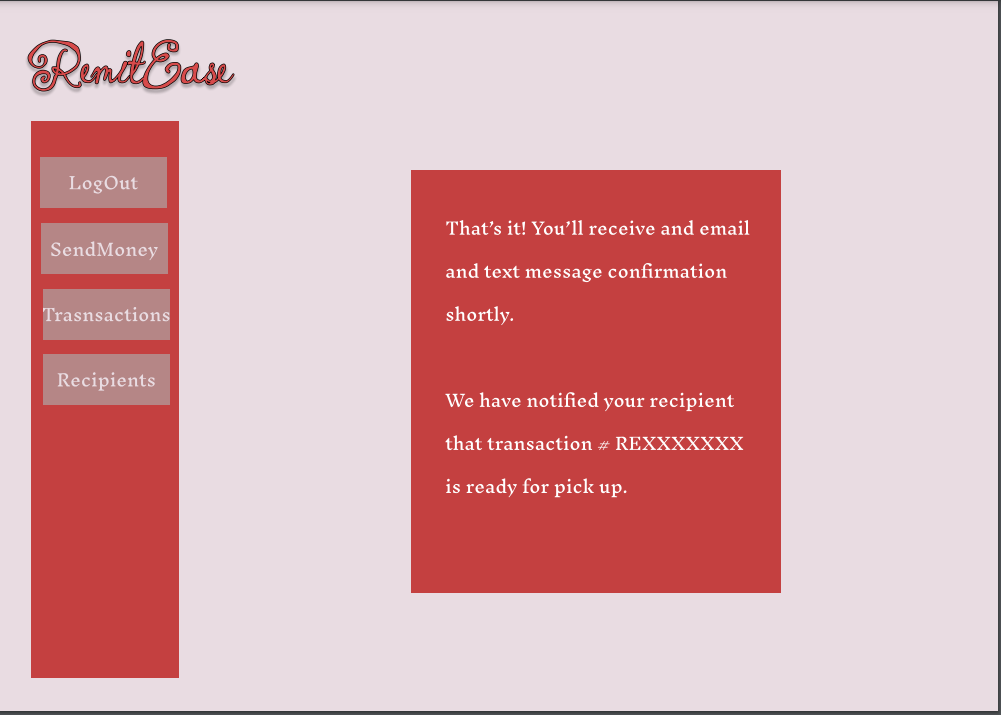
\includegraphics[width=.97\linewidth]{MockUps/SendConfirmation.PNG}
        
        Backend function has processed the transaction. Front end function shows the confirmation.

    \end{landscape}

    \begin{landscape}
        \subsection{Tranasaction History}
        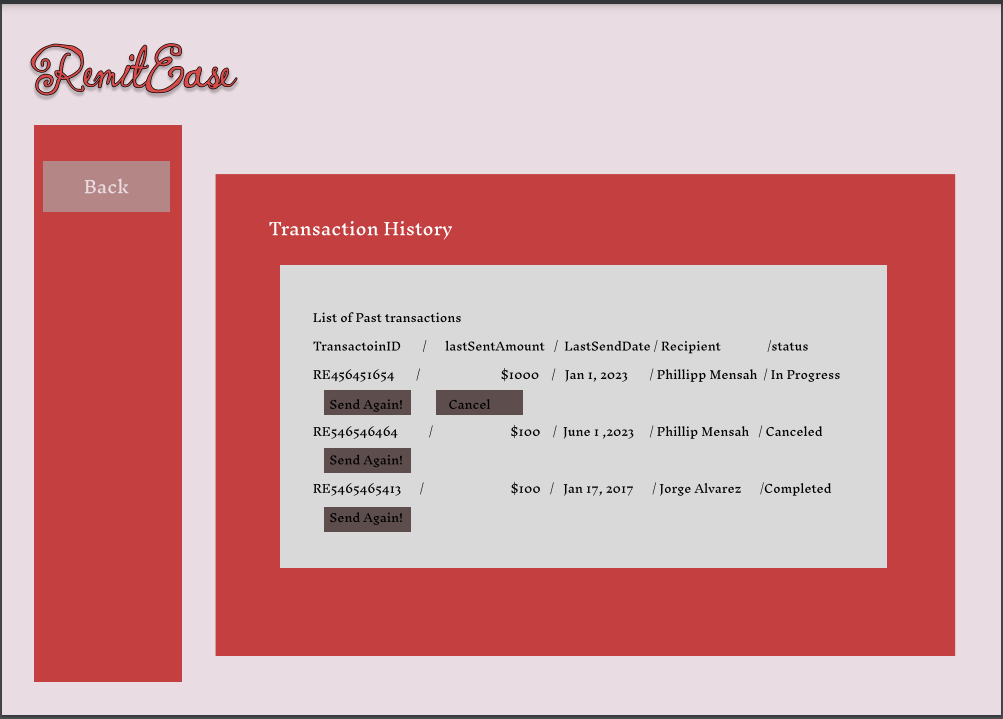
\includegraphics[width=.97\linewidth]{MockUps/TransactionHist.PNG}

       Function to show transaction history and status. Function to send again. Function to cancel pending transaction.
    \end{landscape}
    

    \begin{landscape}
    \subsection{Cancel Confirmation}
        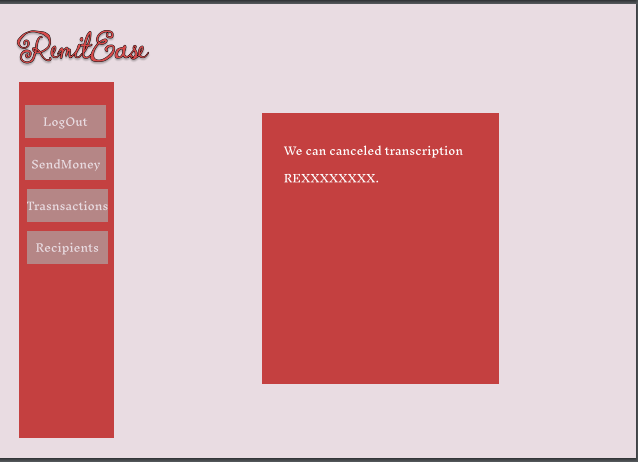
\includegraphics[width=.97\linewidth]{MockUps/CancelConfirmation.PNG}

        Backend has successfully changed the status of the transaction  to cancelled. Front end shows confirmation.
    \end{landscape}

    \begin{landscape}
        
    \section{\colorbox{white!95!black}{Class diagram:}} 



    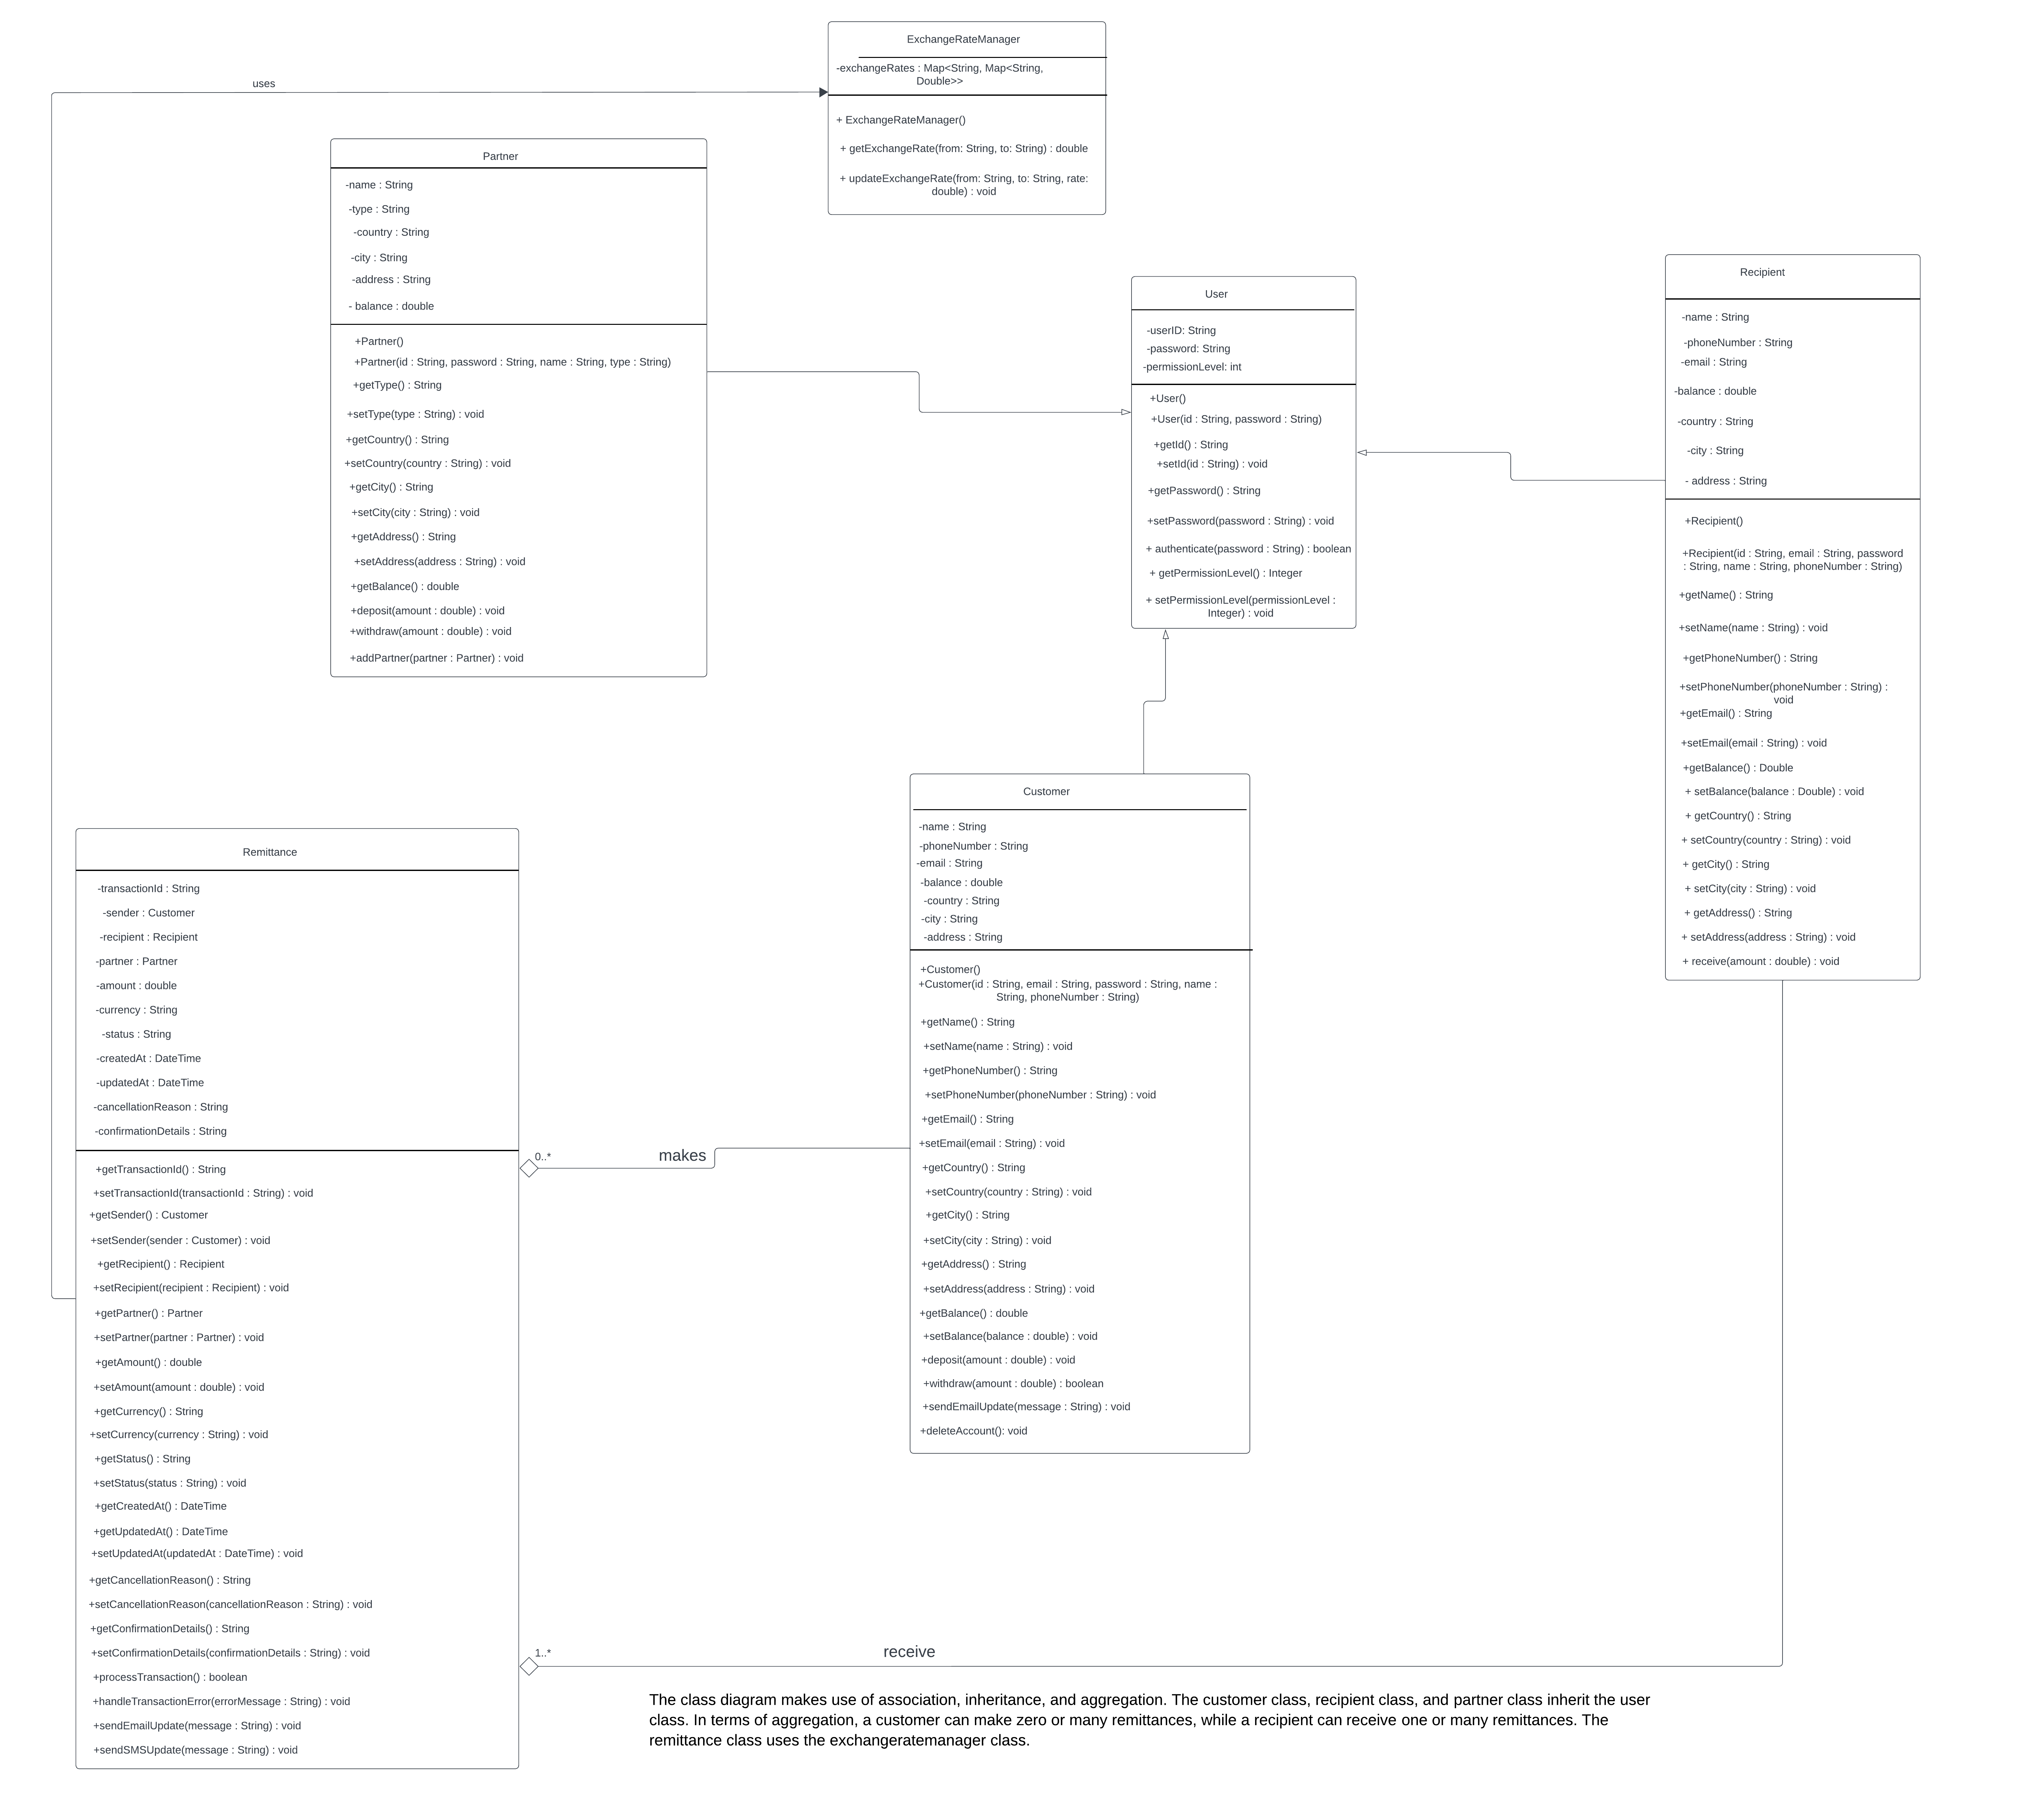
\includegraphics[width=.81\linewidth]{Class Diagram.png}




    \end{landscape}

    
        \subsection{User Class}

        \subsection{Class Diagram}



            \begin{tikzpicture}
                 \umlclass[type=abstract, fill = white]{User}{
                        - id : String \\
                        - password : String \\
                        - permissionLevel : Integer
                    }{
                        + User(id : String, password : String, permissionLevel : Integer) \\
                        + getId() : String \\
                        + setId(id : String) : void \\
                        + getPassword() : String \\
                        + setPassword(password : String) : void \\
                        + getPermissionLevel() : Integer \\
                        + setPermissionLevel(permissionLevel : Integer) : void \\
                        + authenticate(password : String) : boolean
                    }
                
            \end{tikzpicture}

        The user class is used to define user permission levels and authentication.
       
            \subsubsection{Core Attributes:}
            \begin{itemize}
                \item \textbf{\say{id}}: This is a unique identifier for each user. This will link a user to a transaction in the system.
                \item \textbf{\say{password}}: password that allows a user id access to the system.
                \item \textbf{\say{permisionLevel}}: A way to differentiate users based on their roles and actions they can make within the system. 
            \end{itemize}
            \subsubsection{Constructor and Methods:}
            \begin{itemize}
                \item \textbf{getID()}, \textbf{setId(id)} Provide access to a user unique identifier.
                \item \textbf{getPassword()}, \textbf{setPassword(password)}: For management of user password
                \item \textbf{getPermissionLevel()}, \textbf{SetPermissionLevel(permissionLevel)}: Allows the retrieval and update of a users permission level. Regular users have basic permission levels that allow them  to imitate remittances, add recipients, and view their transaction history. Administrator have higher permission that can manage all aspects of the system, such as add new partners. Partners, such as bank or other financial institutions, have permission that allow them to process transactions.
                \item \textbf{authenticate(password)}: Method to verify the input password with the password on file. If match returns boolean to allows access to system.
                
            \end{itemize}

        \subsection{Customer Class Extends user}
            \begin{tikzpicture}
                \umlclass[y=-5, fill = white]{Customer}{
                - name : String \\
                - phoneNumber : String \\
                - email : String \\
                - balance : double \\
                - country : String \\
                - city : String \\
                - address : String
            }{
                + Customer(id : String, email : String, password : String, name : String, phoneNumber : String) \\
                + getName() : String \\
                + setName(name : String) : void \\
                + getPhoneNumber() : String \\
                + setPhoneNumber(phoneNumber : String) : void \\
                + getEmail() : String \\
                + setEmail(email : String) : void \\
                + getCountry() : String \\
                + setCountry(country : String) : void \\
                + getCity() : String \\
                + setCity(city : String) : void \\
                + getAddress() : String \\
                + setAddress(address : String) : void \\
                + getBalance() : double \\
                + setBalance(balance : double) : void \\
                + deposit(amount : double) : void \\
                + withdraw(amount : double) : boolean \\
                + sendEmailUpdate(message : String) : void \\
                + sendSMSUpdate(message : String) : void
                + deleteAccount() : void
            }
            \end{tikzpicture}
            
            \subsubsection{Core Attributes:}
            \begin{itemize}
                \item \textbf{\say{name}}: The customers full name.
                \item \textbf{\say{PhoneNumber}}: Customer Phone number critical for verification purposes and sending notifications.
                \item \textbf{\say{email}}: Primary method of communication for sending transaction confirmations.
                \item \textbf{\say{balance}}: Represents the funds available in the customer's account inside the RemitEase system.
                \item \textbf{\say{country},\say{city}, \say{address}}: Customers location information. 
            \end{itemize}
            \subsubsection{Constructor and Methods:}
            \begin{itemize}
                \item \textbf{Customer(...)}: Initializes a new customer object with customer details. This will be called when a new customer registers with RemitEase system.
                \item \textbf{getName(), setName(name)}: get and set methods for the customer's name.
                \item  \textbf{getPhoneNumber(), setPhoneNumber(PhoneNumber)}:Get and set methods to manage a customer's phone number.
                \item \textbf{getEmail(), setEmail(email)}: Get and set methods to manage the customer's email.
                \item \textbf{getBalance(), setBalance(balance)}: Control the customer's account balance, enabling the system to update funds as transactions are made or received.
                \item \textbf{deposit(), withdraw(amount)}. Methods to add or subtract funds from the customer's balance. Initiated by the customer.
                \item \textbf{sendEmailUpdate(message), sendSMSUpdate(message)}: Send Transaction alerts to the customer.
                \item \textbf{deleteAccount()}: allows the customer to delete his account and personal information.
            \end{itemize}
        
        
        \subsection{Recipient class}
            \begin{tikzpicture}
                \umlclass[x=7,y=-5, fill = white]{Recipient}{
                - name : String \\
                - phoneNumber : String \\
                - email : String \\
                - balance : double \\
                - country : String \\
                - city : String \\
                - address : String
            }{
                + Recipient(id : String, email : String, password : String, name : String, phoneNumber : String) \\
                + getName() : String \\
                + setName(name : String) : void \\
                + getPhoneNumber() : String \\
                + setPhoneNumber(phoneNumber : String) : void \\
                + getEmail() : String \\
                + setEmail(email : String) : void \\
                + getBalance() : Double \\
                + setBalance(balance : Double) : void \\
                + getCountry() : String \\
                + setCountry(country : String) : void \\
                + getCity() : String \\
                + setCity(city : String) : void \\
                + getAddress() : String \\
                + setAddress(address : String) : void \\
                + receive(amount : double) : void \\
            }

            \end{tikzpicture}

            \subsubsection{Core Attributes:}
            \begin{itemize}
               \item \textbf{\say{name}}: The recipients full name.
                \item \textbf{\say{PhoneNumber}}: Recipient Phone number critical for verification purposes and sending notifications.
                \item \textbf{\say{email}}: Primary method of communication for sending transaction confirmations.
                \item \textbf{\say{balance}}: Represents the funds available in the recipient account inside the RemitEase system.
                \item \textbf{\say{country},\say{city}, \say{address}}: Recipient location information. 
            \end{itemize}

            \subsubsection{Constructor and Methods:}
            \begin{itemize}
                \item \textbf{Recipient()}: Initializes a new recipient object with their details.
                \item \textbf{getName(), setName(name)}: and other get/set methods: These methods allow the system to retrieve or update the recipient's information. 
                \item \textbf{receive(amount)}: Method to update the recipient balance and trigger a disbursement of funds.
            \end{itemize}

        \subsection{Partner Class Extends user}
            \begin{tikzpicture}
                \umlclass[x=14,y=-5, fill = white]{Partner}{
                - name : String \\
                - type : String \\
                - country : String \\
                - city : String \\
                - address : String \\
                - balance : double
            }{
                + Partner(id : String, password : String, name : String, type : String) \\
                + getType() : String \\
                + setType(type : String) : void \\
                + getCountry() : String \\
                + setCountry(country : String) : void \\
                + getCity() : String \\
                + setCity(city : String) : void \\
                + getAddress() : String \\
                + setAddress(address : String) : void \\
                + getBalance() : double \\
                + deposit(amount : double) : void \\
                + withdraw(amount : double) : void \\
                + addPartner(partner : Partner) : void \\
             
            }
            
                
            \end{tikzpicture}   

            \subsubsection{Core Attributes:}
            \begin{itemize}
                \item \textbf{\say{name}}:Official name of the partner entity.
                \item \textbf{\say{type}}: Description of the partners business. (e.g Bank, Credit union etc.)
                \item \textbf{\say{country}, \say{city}, \say{address}}: Physical location of the partner.
                \item \textbf{\say{balance}}: Reflects the current balance or funds held by the partner in relation to the remittance system. This could represent pre-funded amounts held to facilitate quick transaction processing or settlements due to/from the remittance service.
            \end{itemize}

            \subsubsection{Constructor and Methods:}
            \begin{itemize}
                \item \textbf{partner()}: Initializes a new partner object with their basic information. This would be used when onboarding a new partner into the remittance system.
                \item \textbf{getType, setType(type)}: Methods to get and set the partner's type, allowing the system to categorize partners and potentially tailor services or interfaces according to the partner's role.
                \item \textbf{getCountry(), setCountry(), getCity(), setCity(), getAddress(), setAddress()}:  Manage the partner's location details. 
                \item \textbf{getBalance(), deposit(amount), withdraw(amount)}: Financial operations to manage the funds associated with the partner.
                \item \textbf{addPartner()}: capability to add another partner entity to the system by the administrator.

            \end{itemize}


        \subsection{Remittance Class}
            \begin{tikzpicture}
            \umlclass[x=7,y=-10, fill = white]{Remittance}{
                - transactionId : String \\
                - sender : Customer \\
                - recipient : Recipient \\
                - partner : Partner \\
                - amount : double \\
                - currency : String \\
                - status : String \\
                - createdAt : DateTime \\
                - updatedAt : DateTime \\
                - cancellationReason : String \\
                - confirmationDetails : String
            }{
                + Remittance(transactionId : String, sender : Customer, recipient : Recipient, partner : Partner, \\
                amount : double, currency : String) \\
                + getTransactionId() : String \\
                + setTransactionId(transactionId : String) : void \\
                + getSender() : Customer \\
                + setSender(sender : Customer) : void \\
                + getRecipient() : Recipient \\
                + setRecipient(recipient : Recipient) : void \\
                + getPartner() : Partner \\
                + setPartner(partner : Partner) : void \\
                + getAmount() : double \\
                + setAmount(amount : double) : void \\
                + getCurrency() : String \\
                + setCurrency(currency : String) : void \\
                + getStatus() : String \\
                + setStatus(status : String) : void \\
                + getCreatedAt() : DateTime \\
                + getUpdatedAt() : DateTime \\
                + setUpdatedAt(updatedAt : DateTime) : void \\
                + getCancellationReason() : String \\
                + setCancellationReason(cancellationReason : String) : void \\
                + getConfirmationDetails() : String \\
                + setConfirmationDetails(confirmationDetails : String) : void \\
                + processTransaction() : boolean \\
                + handleTransactionError(errorMessage : String) : void \\
                + sendEmailUpdate(message : String) : void \\
                + sendSMSUpdate(message : String) : void
            }
            
            \end{tikzpicture}

            \subsubsection{Core Attributes:}
            \begin{itemize}
                \item \textbf{\say{transactionID}}:  A unique identifier for each remittance transaction.
                \item \textbf{\say{sender}}: instance representing the individual or entity sending the money. 
                \item \textbf{\say{recipient}}: The Recipient instance representing the individual or entity receiving the money.
                \item \textbf{\say{partner}}: The Partner entity involved in facilitating the remittance. Partners can be banks, money transfer operators, or other financial institutions that help execute the transfer.
                \item \textbf{\say{amount}}: The total sum of money being sent in the remittance.
                \item \textbf{\say{currency}}: The currency in which the remittance is made. 
                \item \textbf{\say{status}}: Pending, completed or cancelled.
                \item \textbf{\say{createdAt} and \say{updatedAt}}: Timestamps marking when the transaction was created and last updated
                \item \textbf{\say{CancellationReason}}: If the transaction is cancelled, this field stores the reason.
                \item \textbf{\say{confirmDetails:}} Information confirming the transaction's completion, which might include reference numbers, partner details, or timestamps.
                
            \end{itemize}

            \subsubsection{Constructors and Methods:}
            \begin{itemize}
                \item \textbf{Remittance}: The constructor initializes a new Remittance object with essential details like transaction IDs, parties involved, amount, and currency.
                \item \textbf{Getters and Setters}: for each attribute allow the system to retrieve and update the transaction's details as it progresses through different states.
                \item \textbf{processTransaction}: executing the remittance, including validating the transaction, debiting the sender, crediting the recipient, and setting the status to completed.
                \item \textbf{handleTransactionError(errorMessage)}: Handles errors that might occur during the processing of the remittance. i.e insufficient funds.
                \item \textbf{sendEmailUpdate(message)} and \textbf{sendSMSupdate(message)}: Methods for sending transaction updates to relevant parties. 
            \end{itemize}

        \subsection{ExchageRateManager Class}
            \begin{tikzpicture}
              \umlclass[fill=white]{ExchangeRateManager}{
                - exchangeRates : Map<String, Map<String, Double>>
              }{
                + ExchangeRateManager() \\
                + getExchangeRate(from: String, to: String) : double \\
                + updateExchangeRate(from: String, to: String, rate: double) : void
              }
            \end{tikzpicture}

            \subsubsection{Core Attributes}
            \begin{itemize}
                \item \textbf{\say{exchangeRates}}: exchange rate from source currency to target currency. 
            \end{itemize}
                
            \subsubsection{Methods:}
            \begin{itemize}
                \item \textbf{ ExchangeRateManager()}: Constructor
                \item \textbf{getExchangeRate(sourceCurrency, targetCurrency)}: This method provides the current exchange rate between two currencie
                \item \textbf{updateExchangeRate(sourceCurrency, targetCurrency, rate)}:  Allows the remittance system to update the exchange rate between any two given currencies. 
            \end{itemize}

    \section{\colorbox{white!95!black}{File and database design:}}
    Data dictionary for database tables and non-database files. Both relational database and plain text files(s) should be used.
    
        Database will be hosted in MYSQL instance hosted by AWS RDS . At the center of our STAR schema we have the transaction table that stores all information pertaining transactions.

        These tables hold all the information needed for our business logic ensuring security, persistence and granularity of data. That includes details of the sender, recipient and also the partners that facilitate the transfer to the recipient in their home country. There is also a table for transactional data. We have placed the fact transaction table at the center of our star schema with the rest of tables serving as dimensions that augment the meaning of each transaction. This way we hope our data is structure to meet the current business needs as well as future needs such as analytical queries. For example, we should be able to track the growth rate and flow of remittances between countries or regions.

        AS for the file CRUD operations, we will create log exceptions. We limit ourselves to using a Database system for the transaction because of efficiency concerns considering the volume of transactions and real-time data processing. Indexing of data, and transactional integrity are some of of the Database system features not present in plain text files. 

        Below is a comprehensive list of the tables. The schema consists of five main tables built around the requirement of imposed by the class diagram. 
        
        \subsubsection{DimCustomer Table} 
            DimCustomer table table stores information about users of RemitEase. It includes detail such a the user's name, email, phone number, and other essential information 
        \subsubsection{DimPartner Table}
        
            The DimPartner table contains data for partners that are part of the RemitEase international remittance network. We are operating under an assumption no existence of a regulatory body. Thus partners can be but are not limited to banks, financial institutions or natural persons that operate inside the recipient's country. This table contains information about the partner's name, type and location.

        \subsubsection{DimLocation Table}

            This location centralizes physical location address for users, recipients and partners. We put this in a dimension table in order to reduce redundancy of data and decrease access times during queries.

        \subsubsection{DimRecipient Table}

            DimRecipient holds the information for the recipients of the remittance. This included their name, contact information, and location to match them with a remittance partner. 
        \subsubsection{FactRemittance Table}

            FactRemittance table is the core of the system. This table tracks the details of each transaction. This table can include IDs as foreign key link to each dimension table as well as transaction specific attribute such as the amount and currency. 


    See the table below for a comprehensive view of all the tables and their attributes.

        \begin{longtable}{|l|l|l|p{5cm}|}
\hline
\textbf{Table Name} & \textbf{Field Name} & \textbf{Type} & \textbf{Description} \\
\hline
\endhead
% User Table
User & UserId & String & Primary Key, Unique Identifier for User \\
 & Password & String & User's Password \\
\hline
% Customer Table
Customer & CustomerId & String & Primary Key, Foreign Key referencing UserId in User Table \\
 & Name & String & Customer's Name \\
 & PhoneNumber & String & Customer's Phone Number \\
 & Email & String & Customer's Email Address \\
 & Balance & Double & Customer's Account Balance \\
 & Country & String & Customer's Country \\
 & City & String & Customer's City \\
 & Address & String & Customer's Address \\
\hline
% Recipient Table
Recipient & RecipientId & String & Primary Key, Foreign Key referencing UserId in User Table \\
 & Name & String & Recipient's Name \\
 & PhoneNumber & String & Recipient's Phone Number \\
 & Email & String & Recipient's Email Address \\
 & Balance & Double & Recipient's Account Balance \\
 & Country & String & Recipient's Country \\
 & City & String & Recipient's City \\
 & Address & String & Recipient's Address \\
\hline
% Partner Table
Partner & PartnerId & String & Primary Key, Foreign Key referencing UserId in User Table \\
 & Name & String & Partner's Name \\
 & Type & String & Type of Partner (e.g., Bank, Money Transfer Operator) \\
 & Country & String & Partner's Country \\
 & City & String & Partner's City \\
 & Address & String & Partner's Address \\
\hline
% Remittance Table
Remittance & TransactionId & String & Primary Key, Unique Identifier for the Transaction \\
 & SenderId & String & Foreign Key referencing CustomerId in Customer Table \\
 & RecipientId & String & Foreign Key referencing RecipientId in Recipient Table \\
 & PartnerId & String & Foreign Key referencing PartnerId in Partner Table \\
 & Amount & Double & Amount of Money being Transferred \\
 & Currency & String & Currency of the Transaction \\
 & Status & String & Status of the Transaction (e.g., Pending, Completed, Cancelled) \\
 & CreatedAt & DateTime & Date and Time when the Transaction was Created \\
 & UpdatedAt & DateTime & Date and Time when the Transaction was Last Updated \\
 & CancellationReason & String & Reason for Transaction Cancellation (if applicable) \\
 & ConfirmationDetails & String & Details upon Transaction Confirmation \\
\hline
% ExchangeRate Table
ExchangeRate & ExchangeRateId & Integer & Primary Key, Unique Identifier for Exchange Rate Entry \\
 & SourceCurrency & String & Source Currency Code \\
 & TargetCurrency & String & Target Currency Code \\
 & Rate & Double & Exchange Rate between Source and Target Currency \\
 & LastUpdated & DateTime & Date and Time when the Exchange Rate was Last Updated \\
\hline
\caption{Database Schema for Remittance System}
\end{longtable}
        

    \section{\colorbox{white!95!black}{Expectations of project fulfillment:}} 

    Based on the class diagram, we have defined six model classes. The program will design and utilize a controller class. The User Interface (UI) design shows that this program will use a window based application. The following classes will use ArrayLists:
Customer: The system will keep track of multiple customers so we will use ArrayLists to store them.

Recipient: The system will have multiple recipients so will use ArrayLists to store them.

Partners: The system will involve multiple partners so we will use ArrayLists to store them.

Remittance: The system will keep track of multiple remittances and we will use ArrayLists to store them. 
We are going to use a file and database system so we will handle exceptions in the system.
\\ 

\subsubsection{CRUD Operations}
Create: The program allows us to create instances of the customer, recipient, and partner classes in MySQL. The program will create Log exceptions such as error messages to data files.

Read: The program fulfills the Read requirements in CRUD by getting data from the various classes. For instance, in the customer class, the program uses getName, getPhoneNumber, getEmail to retrieve customer information.

Update: The program fulfills the Update requirement in CRUD by setting new values in the various classes. For instance, in the recipient class, setName, setPhoneNumber, setEmail is used to update useful information for the recipient.

Delete: The program allows the user to delete their account. The deleteAccount method in the customer class allows the user to delete their account.

In the final system, there will provide documentation and in line comments for all the model classes and the controller class.


    
    



\end{document}











